\documentclass{article}
%
%
\usepackage{graphicx}
\usepackage{amsmath}
\usepackage{url}
\usepackage{xcolor}
\usepackage{natbib}

%don't label equations that aren't referenced in the text:
\newenvironment{eqnnon}{\begin{equation*}}{\end{equation*}}
\newenvironment{eqnarraynon}{\begin{eqnarray*}}{\end{eqnarray*}}

%numbered citations: no difference between in-text and out-of-text citations:
%\newcommand{\citep}[1]{\cite{#1}}
%\newcommand{\citet}[1]{\cite{#1}}

%\newcommand{\revision}{\color{red}}
\newcommand{\revision}{}

\pagestyle{myheadings}
\markright{P. Mills (2019) \textit{SN Applied Sciences} \textbf{1}(11):1451}

\begin{document}

\title{Solving for multi-class using orthogonal coding matrices}

\author{Peter Mills}

\maketitle

\begin{center}
  %\includegraphics[width=0.6\textwidth]{../../multi2/binary_class_map}
  \includegraphics[width=0.6\textwidth]{binary_class_map}
\end{center}

\section*{Abstract}

	\input{orthogonal_rev1_abstract.txt}


\section{Introduction}

Many methods of statistical classication can only discriminate between two classes. 
Examples include lineear classifiers such as perceptrons and logistic regression \citep{Michie_etal1994}, 
piecewise linear classifiers \citep{Herman_Yeung1992,Mills2018},
as well as support vector machines \citep{kernel_intro}.
There are many ways of generalizing binary classification to 
multi-class.

One should distinguish between multi-class methods that only use a subset
of the binary classifiers, adding more as the algorithm narrows down the
class, and those that use all of the binary classifiers, combining the results
or solving for the class probabilities.
In the former category, we have hierarchical multi-class classifiers 
such as decision trees \citep{Cheong_etal2004,Lee_Oh2003} and decision
directed acyclic graphs (DDACs) \citep{Platt_etal2000}.
In the latter category,
two common methods are one versus one and one versus the rest \citep{Hsu_Lin2002}
These in turn generalize to error-correcting codes (ECC) \citep{Dietterich_Bakiri1995}.

The first application of error-correcting codes used random codes:
the assumption is that if there are enough codes (binary classifiers)
they will adequately span the classes.
Later work focused on optimizing the design of the codes: what type of
codes will best span the classes and produce the most accurate results?
Here we can also distinguish between two type: those that use the data
to help design the codes \citep{Crammer_Singer2002,Zhou_etal2008,Zhong_Cheriet2013}
and those that are independent of the data but use the mathematical 
properties of the codes to aid in the design \citep{Allwein_etal2000,Windeatt_Ghaderi2002,Zhou_etal2019}.
It is these latter type of optimized error-correcting codes we are interested in here.

In error-correcting coding, there is a coding matrix, $A$, that specifies
how the set of multiple classes is partitioned for each binary classifier.
For a given column, 
if members of the $j$th class are to take on a $-1/+1$ for the
binary classifier, then the $j$th row is assigned a $-1/+1$.
If the $j$th class is left out, then the $j$th row is assigned a $0$.
Typically, the class of the test point is determined by the distance between
a row in the matrix and a vector of binary {\it decision functions}:
\begin{equation}
	c(\vec x) = \arg \min_i | \vec a_i - \vec r(\vec x) |
	\label{min_dist}
\end{equation}
where $\vec a_i\in \lbrace -1,0,+1 \rbrace$ 
is the $i$th row of the coding matrix and 
$\vec r$ is a vector of decision functions at {\it test point}, $\vec x$.
If we take the upright brackets as a Euclidean distance and expand:
\begin{eqnnon}
	c = \arg \min_i \sum_j \left ( | \vec a_i | + | \vec r | - 2 \vec a_i  \cdot \vec r_i  \right ) 
\end{eqnnon}
Since $| \vec r |$ is constant over $i$, it may be removed from the expression.
Also, for the purposes of this note,
each row of $A$ has the same number of non-zero entries, hence:
\begin{eqnnon}
	| \vec a_i | = | \vec a_j | = const.
\end{eqnnon}
This is most evident for the case in which each binary classifier partitions
all of the classes so that there are no zeros in $A$
as is the case for the one-versus-the-rest partitioning.
Then (\ref{min_dist}) reduces to a {\it voting} solution:
\begin{equation}
	c = \arg \max A \vec r \label{voting}
\end{equation}
Both \citet{Allwein_etal2000} and \citet{Windeatt_Ghaderi2002} show that to
maximize the accuracy of an error-correcting coding matrix, the distance
between each row, $|\vec a_i - \vec a_j|_{i \ne j}$ should be maximized.
Using the same assumptions, this reduces to:
\begin{eqnnon}
	\min |\vec a_i \cdot \vec a_j|_{i \ne j}
\end{eqnnon}
Note the absolute value prevents degenerate rows.
In other words, the coding matrix, $A$, should be orthogonal.

In this note, we describe a fast and simple algorithm that uses orthogonal coding matrices to solve for the conditional probabilites in multi-class
classification.
There are three reasons to require the conditional probabilities:
\begin{enumerate}
	\item Probabilities provide useful extra information, specifically how accurate a given classification is in absence of knowledge of its true value.
	\item The relationship between the binary probabilities and the
		multi-class probabilities derives uniquely and rigorously from probability theory.
	\item Binary classifier that do not return calibrated probability estimates, but nonetheless supply a continuous decision function are easy to recalibrate so that the decision function more closely resembles a probability \citep{Jolliffe_Stephenson2003,Platt1999}.
\end{enumerate}
Two types of orthogonal ECCs with along three other multi-class 
methods--1 vs. 1, 1 vs. the rest, and random ECCs--will be tested on seven
different datasets to see how they compare in terms of classification speed,
classification accuracy and accuracy of the conditional probabilities.

\section{Algorithm}

We wish to design a set of $n$ binary classifiers, each of which return a 
decision function:
\begin{eqnnon}
r_j(\vec x) = P_j(-1 | \vec x) - P_j(+1 | \vec x)
\label{rdef}
\end{eqnnon}
where $P_j(c | \vec x)$ is the conditional probability of the $c$th class of
the $j$th classifier.
Each binary classifier partitions a set of $m$ classes such that for a
given test point, $\vec x$:
\begin{eqnnon}
	\sum_{i=1}^m a_{ij} p_i = r_j; ~~~ j=[1..n]
\label{multiclass}
\end{eqnnon}
where $A=\lbrace a_{ij} \in \lbrace -1, +1 \rbrace  \rbrace$ is a {\it coding
matrix} and $p_i = p(i | \vec x)$ is the 
conditional  probability of the $i$th class.
In vector notation:
\begin{equation}
	A^T \vec p = \vec r \label{inverse}
\end{equation}
This result derives from the fact that the class probabilities are
additive \citep{Kong_Dietterich1997}.
The more general case where a class can be excluded, that is the coding 
may include zeroes, $a_{ij} \in \lbrace -1, 0, +1\rbrace$,
will not be addressed here. 

Note that this assumes that the binary decision functions, $\vec r$,
estimate the conditional probabilities perfectly.
In practice
there are a set of constraints that must be enforced
because $\vec p$ is only allowed to take on certain values.
Thus, we wish to solve the following minimization problem:
\begin{equation}
	\arg \min_{\vec p} | A^T \vec p - \vec r | \label{minimization}
\end{equation}
\begin{eqnarray}
	\sum_{i=1}^m p_i & = & 1 \label{normalization}\\
	p_i & \ge & 0; ~~~ i=[1..m] \label{nonnegative}
\end{eqnarray}

If $A$ is orthogonal,
\begin{eqnnon}
	A A^T = n I
	\label{orthogonal}
\end{eqnnon}
where $I$ is the $m \times m$ identity matrix,
then the unconstrained minimization problem is easy to solve. 
Note that the voting solution in (\ref{voting}) is now equivalent to
the inverse solution in (\ref{inverse}).
%and also that, unless coding matrix, $A$, is 
%square, $n=m$, it is only orthogonal in one direction.
This allows us to determine the class easily, but we also wish to solve for
the probabilities, $\vec p$, so that none of the constraints in 
(\ref{normalization}) or (\ref{nonnegative}) are violated.
Probabilities are useful for gauging the accuracy of a classification result
when its true value is unknown and for recalibrating an image derived from
statistical classification \citep{Fawcett2006,Mills2009,Mills2011}.

The orthogonality property allows us to reduce the minimization problem 
in (\ref{minimization}) to something much simpler:
\begin{eqnnon}
	\arg \min_{\vec p} | \vec p - \vec p_0 |
\end{eqnnon}
where $\vec p_0 = A \vec r/n$ with the constraints in (\ref{normalization}) and
(\ref{nonnegative}) remaining the same.
Because the system has been rotated and expanded, the non-negativity 
constraints in (\ref{nonnegative}) remain orthogonal, meaning they are 
independent: enforcing one by setting one of the probabilities to zero, 
$p_k=0$ for example, shouldn't otherwise affect the solution.
This still leaves the normalization constraint in (\ref{normalization}):
the problem, now strictly geometrical, is comprised of finding the point nearest $p_0$ on the diagonal hyper-surface that bisects the unit hyper-cube.

Briefly, we can summarize the algorithm as follows:
1. move to the nearest point that satisfies the normalization constraint,
(\ref{normalization}); 2. if one or more of the probabilities is negative,
move to the nearest point that satisfies both 
the normalization constraint
and the non-negativity constraints, (\ref{nonnegative}), for the negative probabilities;
3. repeat step 2.
More formally, let $\vec 1$ be a vector of all $1$'s:
\begin{itemize}
	\item $i:=0$; $m_0:=m$
	\item while $\exists k \, p_{ik} < 0 \lor \vec p_i \cdot \vec 1 \ne 1$:
	\begin{itemize}
		\item if $\vec p_i \cdot \vec 1 \ne 1$ then 
		$\vec p_{i+1} := \vec p_i + (\vec p_i \cdot \vec 1 - 1)/m_i$
		\item let $K$ be the set of $k$ such that $p_{i+1,k} < 0$
		\item for each $k \in K$:
		\begin{itemize}
			\item $p_k:=0$
			\item Remove $k$ from the problem
		\end{itemize}
		\item $m_{i+1}:=m_i-|K|$
		\item $i:=i+1$
	\end{itemize}
\end{itemize}

%\begin{algorithmic}
  \STATE $i:=0$
  \STATE $m_0:=m$
  \WHILE {$\exists k \, p_{ik} < 0$ \OR $\vec p_i \cdot \vec 1 \ne 1$}
    \IF{$\vec p_i \cdot \vec 1 \ne 1$} 
      \STATE{$\vec p_{i+1} := \vec p_i + (\vec p_i \cdot \vec 1 -1)/m_i$}
    \ENDIF
    \STATE let $K$ be the set of $k$ such that $p_{i+1, k} < 0$
    \FORALL{$k \in K$}
       \STATE $p_k:=0$
       \STATE Remove $k$ from the problem
    \ENDFOR
    \STATE $m_{i+1}:=m_i-|K|$
    \STATE $i:=i+1$
  \ENDWHILE 
\end{algorithmic}



Note that resultant direction vectors for each step form an orthogonal set.
For instance, suppose $m_0=4$ and after enforcing the normalization constraint,
the first probability is less than zero, $p_{1,1} < 0$,
then the direction vectors for the two motions are:
\begin{eqnnon}
	\frac{1}{2}[1, 1, 1, 1] \cdot \frac{1}{2\sqrt{3}} [-3, 1, 1, 1] = 0
\end{eqnnon}

More generally, consider the following sequence of vectors:
\begin{eqnnon}
	v_{ij} = \frac{1}{\sqrt{(m-i)^2-2(m-i-1)}} \left \lbrace \begin{array}{rl}
			0; & j < i \\
			-m+i+1; & j=i \\
			1; & j > i
		\end{array} \right .
\end{eqnnon}
where $i \in [1, m]$ and $j \in [1, m]$. \citep{Boyd_Vandenberghe2004}
A nice feature of this method, in addition to being fast,
is that it is divided into two stages: a solution stage and a normalization stage.

\section{Constructing the coding matrix}

\label{construction}

Finding an $A$ such that $A A^T = n I$ and $a_{ij} \in \lbrace -1, 1, \rbrace$
is quite a difficult combinatorial problem.
Work in signal processing may be of limited applicability because coding
matrices are typically comprised of $0$'s and $1$'s 
rather than $-1$'s and $+1$'s \citep{Hedayat_etal1999,Panse_etal2014}.
A further restriction is that
columns must have both positive and negative elements, or:
\begin{equation}
	\left | \sum_{i=0}^m a_{ij} \right | < m;  ~~~ i=[1..n] \label{restriction}
\end{equation}

A simple method of designing an orthogonal $A$ is using harmonic series.
Consider the following matrix for six classes ($m=6$) 
and eight binary classifiers ($n=8$):
\begin{equation}
	A = \left [ \begin{array}{rrrrrrrr}
			 1 & 1 & 1 & 1 & 1 & 1 & 1 & 1 \\
			-1 & -1 & -1 & -1 & 1 & 1 & 1 & 1 \\
			-1 & -1 & 1 & 1 & -1 & -1 & 1 & 1 \\
			-1 & 1 & -1 & 1 & -1 & 1 & -1 & 1 \\
			 1 &  1 & -1 & -1 & -1 & -1 & 1 & 1 \\
			-1 & 1 & 1 & -1 & -1 & 1 & 1 & -1 
	\end{array} \right ]
	\label{harmonic}
\end{equation}
This will limit the size of $m$ relative to $n$; more precisely:
$m \le \lfloor 2 \log_2 n \rfloor$. Moreover, only certain values of $n$
will be admitted: $n=2^t$ where $t$ is a whole number.

The first three rows in (\ref{harmonic}) comprise a Walsh-Hadamard code \citep{Arora_Barak2009}:
all possible permutations are listed.
A square ($n=m$) orthogonal coding matrix is called a Hadamard matrix
\citep{Sylvester1867}.
It can be shown that besides $n=1$ and $n=2$, only Hadamard matrices of size
$n=4t$ exist,  
and it is still unproven that examples exist for all values of $t$
\citep{Hedayat_Wallis1978}.
A very simple, recursive method exists to generate matrices of size $n=t^2$ 
\citep{Hedayat_Wallis1978} but cannot be made to have the property in (\ref{restriction}): 
the matrix includes a both a row and column of only ones.
Such a matrix will include a ``harmonic series'' of the same type as in
(\ref{harmonic}).

%Noting which versions of $A$ are degenerate (equivalent) can help us whittle
%away at the problem:
%\begin{itemize}
%	\item $-A$ is equivalent to $A$
%	\item re-arranging either the rows or columns of $A$ makes an equivalent $A$: $T_{ij} A$ or $A T_{ij}^T$ are both equivalent to $A$ where $T_{ij}$ is the elementary matrix which exchanges rows $i$ and $j$
%\end{itemize}

To compute the results in this note, orthogonal coding matrices were generated
using a ``greedy'' algorithm.
We choose $n$ to be the smallest multiple of $4$ equal to or larger than $m$.
and start with an empty matrix.
Candidate vectors containing both positive and negative elements 
are chosen at random to comprise a row of the matrix but never repeated.
If the candidate vector is orthogonal to existing rows, then it is added to the matrix.
New candidates are tested until the matrix is filled or we run out of permutations.
A full matrix is almost always returned especially if $m<n$.
The matrix is then checked to ensure that 
each column contains both positive and negative elements.
Note that the whole process can be repeated as many times as necessary.

More work will need to be done to find efficient methods
of generating these matrices
if they are to be efficiently applied to problems with a large number of classes.


\section{Results}

\begin{table*}
\caption{Solution time, uncertainty coefficient and Brier score for six different datasets using five different coding matrices: 1 vs. 1, 1 vs. the rest, random error correcting codes, orthogonal "strict" coding, and orthogonal "non-strict" coding. Logistic regression is used as the base binary classifier.}\label{class_results_lin}
\begin{tabular}{ll|llll}
\hline
Dataset & Method & time (s) & sol. only (s) & U.C. & Brier score \\
\hline\hline
	pendigits & 1 vs. 1 & $       0.489\pm   0.006$ & $0.410\pm0.004$ & $     \mathbf{0.956\pm   0.006}$ & $   \mathbf{0.0566\pm   0.003}$\\
 & 1 vs. rest & $       0.118\pm   0.0042$ & $0.0823\pm0.0011$ & $       0.864\pm    0.008$ & $    0.113\pm   0.002$\\
 & ECC & $        0.18\pm    0.01$ & $0.136\pm0.007$ & $     0.723\pm    0.026$ & $    0.180\pm   0.008$\\
	& Ortho. 1 & $       \mathbf{0.048\pm   0.004}$ & $\mathbf{0.01095\pm8e-5}$ & $     0.785\pm   0.010$ & $    0.172\pm   0.002$\\
 & Ortho. 2 & $       0.24\pm    0.01$ & $0.185\pm0.010$ & $     0.862\pm     0.010$ & $    0.123\pm    0.009$\\
\hline
	sat & 1 vs. 1 & $       0.092\pm   0.004$ & $0.067\pm0.001$ & $     \mathbf{0.736\pm   0.009}$ & $    \mathbf{0.176\pm   0.004}$\\
 & 1 vs. rest & $       0.033\pm   0.0048$ & $0.0202\pm2e-4$ & $     0.677\pm   0.007$ & $    0.204\pm   0.002$\\
 & ECC & $       0.043\pm   0.0048$ & $0.0274\pm6e-4$ & $     0.637\pm    0.025$ & $    0.217\pm   0.009$\\
	& Ortho. 1 & $       \mathbf{0.019\pm   0.006}$ & $\mathbf{0.00422\pm8e-5}$ & $     0.665\pm   0.009$ & $    0.210\pm   0.002$\\
 & Ortho. 2 & $       0.046\pm   0.005$ & $0.0271\pm0.0017$ & $     0.688\pm    0.018$ & $    0.197\pm     0.010$\\
\hline
	segment & 1 vs. 1 & $        0.04\pm  5.9e-06$ & $0.0336\pm4e-4$ & $     \mathbf{0.911\pm   0.009}$ & $   \mathbf{0.0987\pm   0.0057}$\\
 & 1 vs. rest & $       0.012\pm   0.0042$ & $0.0094\pm2e-4$ & $     0.868\pm   0.010$ & $    0.144\pm   0.004$\\
 & ECC & $       0.016\pm   0.0052$ & $0.0124\pm4e-4$ & $     0.803\pm     0.040$ & $    0.179\pm     0.020$\\
	& Ortho. 1 & $       \mathbf{0.004\pm   0.005}$ & $\mathbf{0.00168\pm6e-5}$ & $     0.84863\pm    0.015$ & $    0.166\pm    0.004$\\
 & Ortho. 2 & $        0.02\pm  2.9e-06$ & $0.0147\pm0.0012$ & $     0.880\pm    0.018$ & $    0.127\pm   0.008$\\
\hline
	shuttle & 1 vs. 1 & $       1.10\pm    0.03$ & $0.867 \pm 0.014$ & $     \mathbf{0.796\pm    0.013}$ & $   \mathbf{0.0824\pm   0.0017}$\\
 & 1 vs. rest & $       0.33\pm    0.01$ & $0.185\pm0.003$ & $     0.605\pm     0.010$ & $    0.13412\pm  0.0006$\\
 & ECC & $       0.42\pm    0.01$ & $0.265\pm0.011$ & $     0.535\pm     0.120$ & $    0.1436\pm    0.026$\\
	& Ortho. 1 & $       \mathbf{0.183\pm   0.005}$ & $\mathbf{0.042\pm0.001}$ & $     0.593\pm   0.006$ & $    0.131\pm   0.002$\\
 & Ortho. 2 & $        0.48\pm    0.03$ & $0.31\pm0.03$ & $     0.710\pm    0.095$ & $    0.101\pm    0.024$\\
\hline
urban & 1 vs. 1 & $       0.031\pm   0.003$ & $0.0185\pm 1e-4$ & $     0.693\pm    0.026$ & $    \mathbf{0.188\pm   0.006}$\\
 & 1 vs. rest & $       \mathbf{0.007\pm   0.005}$ & $0.0052\pm 4e-4$ & $     0.667\pm    0.018$ & $    0.204\pm   0.004$\\
 & ECC & $       0.009\pm   0.003$ & $0.0068 \pm 4e-4$ & $     0.647\pm    0.031$ & $    0.210\pm   0.008$\\
 & ortho. 1 & $       \mathbf{0.007\pm   0.005}$ & $\mathbf{0.00064 \pm 4e-5}$ & $     0.674\pm    0.016$ & $    0.206\pm   0.004$\\
	& ortho. 2 & $       0.014\pm   0.005$ & $0.0082\pm 6e-4$ & $     \mathbf{0.693\pm    0.017}$ & $    0.198\pm   0.006$\\
\hline
	usps & 1 vs. 1 & $       0.63\pm    0.01$ & $0.347\pm0.005$ & $     \mathbf{0.898\pm     0.010}$ & $   \mathbf{0.0827\pm   0.0022}$\\
 & 1 vs. rest & $       0.152\pm   0.004$ & $0.0704\pm9e-4$ & $     0.840\pm   0.007$ & $    0.112\pm   0.003$\\
 & ECC & $       0.205\pm   0.005$ & $0.112\pm0.005$ & $     0.769\pm    0.021$ & $    0.1416\pm    0.006$\\
	& Ortho. 1 & $         \mathbf{0.1\pm  2.1e-05}$ & $\mathbf{0.0096\pm5e-4}$ & $     0.815\pm   0.009$ & $    0.132\pm   0.002$\\
 & Ortho. 2 & $       0.30\pm    0.02$ & $0.16\pm0.01$ & $      0.846\pm    0.015$ & $    0.112\pm   0.004$\\
\hline
	vehicle & 1 vs. 1 & $       0.002\pm   0.004$ & $0.00436\pm8e-5$ & $      \mathbf{0.685\pm    0.041}$ & $    \mathbf{0.245\pm    0.011}$\\
 & 1 vs. rest & $           0$ & $0.00142\pm6e-5$ & $     0.654\pm    0.037$ & $    0.263\pm   0.006$\\
 & ECC & $           0$ & $0.00143\pm8e-5$ & $     0.599\pm    0.049$ & $    0.279\pm    0.013$\\
	& Ortho. 1 & $           0$ & $\mathbf{0.00043\pm3e-5}$ & $     0.656\pm    0.038$ & $    0.263\pm   0.007$\\
 & Ortho. 2 & $           0$ & $0.0014\pm0.0001$ & $     0.636\pm    0.042$ & $    0.263\pm    0.019$\\
\hline
\end{tabular}

\end{table*}

\begin{table*}
\caption{Solution time, uncertainty coefficient and Brier score for six different datasets using five different coding matrices: 1 vs. 1, 1 vs. the rest, random error correcting codes, orthogonal "strict" coding, and orthogonal "non-strict" coding. A support vector machine is used as the base binary classifier.}\label{class_results_svm}
\begin{tabular}{|ll|llll|}
\hline
Dataset & Method & time (s) & sol. only (s) & U.C. & Brier score \\
\hline\hline
	shuttle & 1 vs. 1 & $       6.3\pm        1.0$ & $0.98\pm0.06$ & $      \mathbf{0.982\pm   0.003}$ & $   \mathbf{0.0182\pm   0.0015}$\\
	& 1 vs. rest & $       \mathbf{6.0\pm      1.6}$ & $0.26\pm0.03$ & $     0.978\pm   0.006$ & $   0.02147\pm   0.0011$\\
 & ECC & $       12.4\pm      5.7$ & $0.43\pm0.10$ & $     0.878\pm     0.210$ & $   0.0731\pm      0.100$\\
	& ortho. 1 & $      10.0\pm      4.7$ & $\mathbf{0.09\pm0.03}$ & $     0.974\pm    0.003$ & $   0.0222\pm    0.0010$\\
 & ortho. 2 & $       6.6\pm      1.6$ & $0.40\pm0.04$ & $     0.978\pm   0.002$ & $   0.0230\pm   0.0068$\\
\hline
	segment & 1 vs. 1 & $       0.178\pm    0.045$ & $0.034\pm0.001$ & $     0.923\pm   0.007$ & $   \mathbf{0.0882\pm   0.0053}$\\
 & 1 vs. rest & $       0.111\pm    0.032$ & $0.0102\pm0.0005$ & $      0.919\pm   0.007$ & $   0.0938\pm   0.0051$\\
 & ECC & $       0.133\pm    0.067$ & $0.014\pm0.001$ & $     0.915\pm    0.013$ & $   0.0938\pm   0.0071$\\
	& ortho. 1 & $       0.163\pm    0.072$ & $0.0018\pm0.0001$ & $     \mathbf{0.925\pm   0.008}$ & $   0.0890\pm   0.0048$\\
 & ortho. 2 & $       0.112\pm    0.032$ & $0.015\pm0.001$ & $     0.919\pm    0.012$ & $   0.0883\pm    0.0050$\\
\hline
	sat & 1 vs. 1 & $       \mathbf{1.39\pm     0.35}$ & $0.077\pm0.009$ & $     \mathbf{0.800\pm     0.010}$ & $    \mathbf{0.145\pm   0.003}$\\
 & 1 vs. rest & $       1.70\pm     0.54$ & $0.028\pm0.005$ & $     0.786\pm   0.009$ & $    0.153\pm   0.003$\\
 & ECC & $       3.2\pm      1.6$ & $0.04\pm0.01$ & $     0.787\pm    0.011$ & $    0.152\pm   0.004$\\
	& ortho. 1 & $       3.8\pm        1.0$ & $\mathbf{0.008\pm0.003}$ & $     0.792\pm    0.011$ & $    0.149\pm   0.003$\\
 & ortho. 2 & $        1.79\pm     0.52$ & $0.034\pm0.007$ & $     0.789\pm   0.009$ & $    0.150\pm   0.004$\\
\hline
	pendigits & 1 vs. 1 & $       1.07\pm     0.14$ & $0.409\pm0.006$ & $     \mathbf{0.985\pm   0.003}$ & $   \mathbf{0.0319\pm   0.0024}$\\
	& 1 vs. rest & $       \mathbf{0.84\pm    0.10}$ & $0.082\pm0.002$ & $     0.981\pm   0.003$ & $   0.0361\pm   0.0034$\\
 & ECC & $       3.20\pm     0.86$ & $0.13\pm0.01$ & $     0.975\pm   0.004$ & $   0.0412\pm   0.0032$\\
	& ortho. 1 & $       2.13\pm     0.89$ & $\mathbf{0.013\pm0.002}$ & $     0.979\pm   0.004$ & $   0.0382\pm   0.0026$\\
	& ortho. 2 & $       1.17\pm     0.28$ & $0.20\pm0.01$ & $      \mathbf{0.982\pm   0.004}$ & $   0.0354\pm   0.0034$\\
\hline
	usps & 1 vs. 1 & $        33.9\pm       17.0$ & $0.42\pm0.02$ & $     \mathbf{0.929\pm   0.006}$ & $   \mathbf{0.0664\pm   0.0023}$\\
	& 1 vs. rest & $      \mathbf{22.9\pm      7.6}$ & $0.110\pm0.009$ & $     0.921\pm   0.005$ & $   0.0732\pm    0.0020$\\
 & ECC & $      73.0\pm       29.0$ & $0.150\pm0.009$ & $     0.915\pm    0.006$ & $    0.0754\pm   0.0022$\\
	& ortho. 1 & $      70.1\pm       29.0$ & $\mathbf{0.018\pm0.003}$ & $     0.922\pm   0.006$ & $   0.0712\pm   0.0018$\\
 & ortho. 2 & $      34.8\pm       16.0$ & $0.21\pm0.02$ & $     0.920\pm   0.008$ & $   0.0707\pm   0.0027$\\
\hline
	vehicle & 1 vs. 1 & $       0.047\pm    0.013$ & $0.00465\pm8e-5$ & $     0.635\pm    0.023$ & $    \mathbf{0.272\pm   0.007}$\\
 & 1 vs. rest & $       0.055\pm    0.016$ & $0.0016\pm0.001$ & $     0.625\pm    0.033$ & $    0.277\pm   0.009$\\
 & ECC & $       0.053\pm    0.024$ & $0.0017\pm0.0002$ & $     0.610\pm    0.061$ & $    0.282\pm    0.011$\\
	& ortho. 1 & $        0.05\pm    0.018$ & $\mathbf{0.00050\pm3e-5}$ & $     0.621\pm    0.032$ & $    0.277\pm    0.009$\\
	& ortho. 2 & $       \mathbf{0.042\pm   0.006}$ & $0.00155\pm9e-5$ & $     \mathbf{0.639\pm    0.025}$ & $    0.278\pm   0.009$\\
\hline
\end{tabular}

\end{table*}

\begin{table*}
\caption{Solution time, uncertainty coefficient and Brier score for six different datasets using five different coding matrices: 1 vs. 1, 1 vs. the rest, random error correcting codes, orthogonal "strict" coding, and orthogonal "non-strict" coding. A piecewise linear classifier is used as the base binary classifier.}\label{class_results_acc}
\begin{tabular}{|ll|llll|}
\hline
Dataset & Method & time (s) & sol. only (s) & U.C. & Brier score \\
\hline\hline
	pendigits & 1 vs. 1 & $       1.71\pm    0.08$ & $0.45\pm0.02$ & $     \mathbf{0.977\pm   0.005}$ & $   \mathbf{0.0383\pm   0.003}$\\
	& 1 vs. rest & $       \mathbf{0.62\pm    0.02}$ & $0.088\pm0.004$ & $     0.967\pm   0.006$ & $   0.0539\pm   0.0021$\\
 & ECC & $       0.77\pm    0.02$ & $0.14\pm0.01$ & $     0.955\pm    0.011$ & $   0.0603\pm   0.0061$\\
	& ortho. 1 & $       0.64\pm    0.01$ & $\mathbf{0.0122\pm0.0005}$ & $     0.961\pm   0.006$ & $   0.0560\pm   0.0037$\\
 & ortho. 2 & $       1.3\pm      0.1$ & $0.21\pm0.02$ & $     0.969\pm   0.007$ & $   0.0471\pm   0.0033$\\
	\hline
	sat & 1 vs. 1 & $       1.97\pm    0.07$ & $0.098\pm0.02$ & $     \mathbf{0.783\pm   0.009}$ & $    \mathbf{0.159\pm   0.005}$\\
	& 1 vs. rest & $       \mathbf{1.17\pm    0.03}$ & $0.035\pm0.007$ & $     0.768\pm    0.012$ & $    0.168\pm   0.003$\\
 & ECC & $       1.54\pm    0.05$ & $0.045\pm0.01$ & $     0.765\pm    0.013$ & $    0.165\pm    0.004$\\
	& ortho. 1 & $       1.50\pm    0.04$ & $\mathbf{0.010\pm0.004}$ & $     0.776\pm   0.009$ & $    0.162\pm   0.004$\\
 & ortho. 2 & $       1.6\pm     0.2$ & $0.047\pm0.01$ & $     0.763\pm   0.009$ & $    0.169\pm   0.010$\\
	\hline
	segment & 1 vs. 1 & $        0.170\pm   0.005$ & $0.0353\pm4e-4$ & $     \mathbf{0.911\pm    0.011}$ & $   \mathbf{0.096\pm   0.005}$\\
	& 1 vs. rest & $       \mathbf{0.099\pm   0.0032}$ & $0.0104\pm4e-4$ & $     0.88268\pm    0.019$ & $    0.119\pm   0.004$\\
 & ECC & $       0.113\pm   0.005$ & $0.015\pm0.001$ & $     0.888\pm    0.026$ & $     0.116\pm   0.010$\\
	& ortho. 1 & $       \mathbf{0.099\pm   0.003}$ & $\mathbf{0.00190\pm5e-5}$ & $     0.896\pm    0.011$ & $    0.115\pm   0.005$\\
 & ortho. 2 & $        0.15\pm    0.01$ & $0.0160\pm7e-4$ & $     0.910\pm    0.011$ & $    0.103\pm   0.007$\\
	\hline
	shuttle & 1 vs. 1 & $       4.398\pm    0.093$ & $0.90\pm0.03$ & $     \mathbf{0.981\pm   0.010}$ & $   0.0274\pm    0.0110$\\
	& 1 vs. rest & $       \mathbf{2.51\pm    0.04}$ & $0.217\pm0.006$ & $     0.967\pm    0.028$ & $   0.0315\pm   0.0083$\\
 & ECC & $       2.89\pm     0.06$ & $0.28\pm0.02$ & $     0.972\pm    0.005$ & $   0.0313\pm   0.0044$\\
	& ortho. 1 & $       2.63\pm    0.04$ & $\mathbf{0.045\pm0.001}$ & $     0.976\pm   0.002$ & $    \mathbf{0.0261\pm   0.0010}$\\
 & ortho. 2 & $       3.7\pm     0.3$ & $0.35\pm0.03$ & $     0.976\pm   0.004$ & $   0.0270\pm   0.0043$\\
	\hline
	urban & 1 vs. 1 & $        0.94\pm    0.02$ & $0.023\pm0.001$ & $     \mathbf{0.724\pm    0.019}$ & $    \mathbf{0.172\pm    0.009}$\\
	& 1 vs. rest & $       \mathbf{0.23\pm    0.01}$ & $0.005\pm0.001$ & $     0.698\pm    0.032$ & $    0.184\pm    0.011$\\
 & ECC & $       0.314\pm   0.008$ & $0.008\pm0.001$ & $     0.692\pm    0.028$ & $    0.184\pm   0.006$\\
	& ortho. 1 & $       0.31\pm    0.01$ & $\mathbf{0.0012\pm4e-4}$ & $     0.717\pm    0.022$ & $    0.176\pm   0.008$\\
 & ortho. 2 & $       0.44\pm    0.03$ & $0.011\pm0.001$ & $      0.719\pm    0.034$ & $    0.176\pm    0.015$\\
	\hline
	usps & 1 vs. 1 & $      14.4\pm     0.2$ & $0.41\pm0.02$ & $     \mathbf{0.914\pm   0.005}$ & $   \mathbf{0.075\pm   0.002}$\\
	& 1 vs. rest & $       \mathbf{6.2\pm     0.1}$ & $0.08\pm0.01$ & $     0.8972\pm   0.007$ & $     0.101\pm   0.002$\\
 & ECC & $       7.5\pm     0.1$ & $0.14\pm0.02$ & $     0.881\pm   0.006$ & $   0.095\pm   0.003$\\
	& ortho. 1 & $       7.3\pm      0.1$ & $\mathbf{0.014\pm0.004}$ & $     0.897\pm   0.006$ & $   0.089\pm   0.002$\\
 & ortho. 2 & $      12\pm        1$ & $0.20\pm0.02$ & $     0.899\pm   0.008$ & $   0.084\pm   0.003$\\
	\hline
	vehicle & 1 vs. 1 & $       0.017\pm   0.005$ & $0.0044\pm1e-4$ & $     \mathbf{0.628\pm    0.038}$ & $      \mathbf{0.273\pm    0.007}$\\
 & 1 vs. rest & $       0.017\pm   0.005$ & $0.00156\pm8e-5$ & $      0.607\pm    0.036$ & $     0.282\pm   0.007$\\
 & ECC & $        0.02\pm  2.9e-06$ & $0.00158\pm5e-5$ & $     0.602\pm    0.067$ & $    0.283\pm    0.014$\\
	& ortho. 1 & $       \mathbf{0.015\pm   0.005}$ & $\mathbf{0.00046\pm1e-5}$ & $     0.614\pm    0.026$ & $    0.281\pm   0.007$\\
 & ortho. 2 & $       0.016\pm   0.005$ & $0.0015\pm1e-4$ & $      0.597\pm    0.041$ & $    0.287\pm    0.011$\\
\hline
\end{tabular}


\end{table*}

Orthogonal error-correcting codes were tested on six different datasets:
two for digit recognition--``pendigits'' \citep{Alimoglu1996} and
``usps'' \citep{Hull1994}; the space shuttle control dataset--``shuttle''
\citep{King_etal1995}; a satellite land recognition
dataset--``sat''; a similar dataset for image recognition--``segment'';
and a dataset for vehicle recognition--``vehicle'' \citep{Siebert1987}.
The last four are borrowed from the ``statlog'' project \citep{King_etal1995,Michie_etal1994}.

The method was compared with random error-correcting codes using the same
number of codes or matrix rows, $m$.
Random codes were solved using a constrained linear least squares method based
on the Karesh-Kuhn-Tucker conditions \citep{Lawson_Hanson1995}.
Both techniques were applied to support vector machines (SVMs) trained using
LIBSVM \citep{Chang_Lin2011}.
Partitions were trained separately then combined by finding the union of
sets of support vectors for each partition.
By indexing into the combined list of support vectors, the algorithms are
optimized in both space and time \citep{Chang_Lin2011}.

The same parameters were used for both the random and orthogonal codes and 
for all partitions.
All datasets were trained using  ``radial basis function'' (Gaussian)
kernels of differing widths.

Results are shown in Table \ref{class_results}.
Confidence limits represent standard deviations over 20 trials using
different, randomly chosen coding matrices.
For each trial, datasets were randomly separated into 70\% training and 30\%
test.
``U.C'' stands for uncertainty
coefficient, a skill score based on Shannon's channel capacity
\citep{Shannon,Press_etal1992,Mills2011} that has many advantage over simple
fraction of correct guesses or ``accuracy''.
Probabilities are validated with the Brier score 
which is root-mean-square
error measured against the truth of the class as a 0 or 1 value
\citep{Brier1950,Jolliffe_Stephenson2003}.

For all of the datasets tested, orthogonal coding matrices provide a small but
significant improvement over random coding matrices in both classification
accuracy and in the accuracy of the conditional probabilities.
This is in line with the literature as in \citet{Dietterich_Bakiri1995,Windeatt_Ghaderi2002}.
Results are also more consistent for the orthogonal codes as given by the
calculated error bars.

Also as expected, solution times are
considerably faster for the orthogonal coding matrices.
Depending on the problem and classification method, this may or may not
be significant.
Since SVM is a relatively slow classifier, solution times
are a minor portion of the total.
For fast classifiers such as a linear classifier or perceptron,
solving the constrained optimization problem for the probabilities
could easily comprise the bulk of classification times.
Note that for both methods under examination, time to perform the binary
classifications should be roughly equivalent.

As predicted, solving for multi-class using orthogonal coding matrices 
is more accurate than the equivalent problem using random coding matrices.
While the difference is small,
the method is simple and elegant and
may suggest new directions in the search for more efficient and
accurate multi-class classification algorithms.



\appendix

\section*{acknowledgements}
Thanks to Chih-Chung Chan and Chih-Jen Lin of the National Taiwan University
for data from the LIBSVM archive and also to David Aha and the curators of
the UCI Machine Learning Repository for statistical classification datasets.

	The LIBSVM software libraries can be found: \url{https://www.csie.ntu.edu.tw/~cjlin/libsvm/}.
	The LIBLINEAR software libraries can be found: \url{https://www.csie.ntu.edu.tw/~cjlin/liblinear/}.
	Software for performing multi-class classification using orthogonal error correcting codes, and many others, can be found: \url{https://www.github.com/peteysoft/libmsci}.

\bibliographystyle{apa}
%\bibliographystyle{unsrt}

%\newpage
%\addcontentsline{toc}{section}{References}

\bibliography{../../agf_bib,../orthogonal,../../pwl,../../svm_accel/svm_accel,../../datasets}   % name your BibTeX data base

\end{document}

